%%%%%% Run at command line, run
%%%%%% xelatex grad-sample.tex 
%%%%%% for a few times to generate the output pdf file
\documentclass[12pt,oneside,openright,a4paper]{cpe-english-project}
%%%%%% add package for gantt chart
\usepackage{xcolor,colortbl}
\usepackage{forloop}
\newcounter{loopcntr}
\newcommand{\rpt}[2][1]{%
  \forloop{loopcntr}{0}{\value{loopcntr}<#1}{#2}%
}
\newcommand{\on}[1][1]{
  \forloop{loopcntr}{0}{\value{loopcntr}<#1}{&\cellcolor{gray}}
}
\newcommand{\off}[1][1]{
  \forloop{loopcntr}{0}{\value{loopcntr}<#1}{&}
}

%%%%% add package multirole for table
\usepackage{multirow}

\defaultfontfeatures{Mapping=tex-text,Scale=1.0,LetterSpace=0.0}
\setmainfont[Scale=1.0,LetterSpace=0,WordSpace=1.0,FakeStretch=1.0]{Times New Roman}
%\setmathfont(Digits)[Scale=1.0,LetterSpace=0,FakeStretch=1.0]{Times New Roman}


%%%%%%%%%%%%%%%%%%%%%%%%%%%%%%%%%%%%%%%%%%%%%%%%%%%%%%%%%%%%%%%%%%%
% Customize below to suit your needs 
% The ones that are optional can be left blank. 
%%%%%%%%%%%%%%%%%%%%%%%%%%%%%%%%%%%%%%%%%%%%%%%%%%%%%%%%%%%%%%%%%%%
% First line of title
\def\disstitleone{Project No. 50}   
% Second line of title
\def\disstitletwo{NKR: On top scheduler for Apache Mesos}   
% Your first name and lastname
\def\dissauthor{Ms.Pasinee Santivorranant}   % 1st member
%%% Put other group member names here ..
\def\dissauthortwo{Mr.Supapat Sri-on}   % 2nd member (optional)
\def\dissauthorthree{Ms.Parattha Weerapong}   % 3rd member (optional)


% The degree that you're persuing..
\def\dissdegree{Bachelor of Engineering} % Name of the degree
\def\dissdegreeabrev{B.Eng} % Abbreviation of the degree
\def\dissyear{2020}                   % Year of submission
\def\thaidissyear{2563}               % Year of submission (B.E.)

%%%%%%%%%%%%%%%%%%%%%%%%%%%%%%%%%%%%%%%%%%%%
% Your project and independent study committee..
%%%%%%%%%%%%%%%%%%%%%%%%%%%%%%%%%%%%%%%%%%%%
\def\dissadvisor{Asst Prof.Rajchawit Sarochawikasit}  % Advisor
%%% Leave it empty if you have no Co-advisor
\def\disscoadvisor{}  % Co-advisor
\def\disscommitteetwo{Asst Prof. Dr. Khajonpong Akkarajitsakul}  % 3rd committee member (optional)
\def\disscommitteethree{Asst Prof. Dr. Phond Phunchongharn}   % 4th committee member (optional) 
\def\disscommitteefour{Asst Prof. Sanan Srakaew}    % 5th committee member (optional) 

\def\worktype{Project} %%  Project or Independent study
\def\disscredit{3}   %% 3 credits or 6 credits


\def\fieldofstudy{Computer Engineering} 
\def\department{Computer Engineering} 
\def\faculty{Engineering}

\def\thaifieldofstudy{วิศวกรรมคอมพิวเตอร์} 
\def\thaidepartment{วิศวกรรมคอมพิวเตอร์} 
\def\thaifaculty{วิศวกรรมศาสตร์}
 
\def\appendixnames{Appendix} %%% Appendices or Appendix

\def\thaiworktype{ปริญญานิพนธ์} %  Project or research project % 
\def\thaidisstitleone{หัวข้อปริญญานิพนธ์บรรทัดแรก}
\def\thaidisstitletwo{หัวข้อปริญญานิพนธ์บรรทัดสอง}
\def\thaidissauthor{นางสาวภาสินี สันติวรนันท์}
\def\thaidissauthortwo{นายศุภพัฒน์ ศรีอ่อน} %Optional
\def\thaidissauthorthree{นางสาวปรัษฐา วีระพงษ์} %Optional

\def\thaidissadvisor{ผศ.ดร.ราชวิชช์ สโรชวิกสิต}
%% Leave this empty if you have no co-advisor
\def\thaidisscoadvisor{} %Optional
\def\thaidissdegree{วิศวกรรมศาสตรบัณฑิต}

% Change the line spacing here...
\linespread{1.15}

%%%%%%%%%%%%%%%%%%%%%%%%%%%%%%%%%%%%%%%%%%%%%%%%%%%%%%%%%%%%%%%%
% End of personal customization.  Do not modify from this part 
% to \begin{document} unless you know what you are doing...
%%%%%%%%%%%%%%%%%%%%%%%%%%%%%%%%%%%%%%%%%%%%%%%%%%%%%%%%%%%%%%%%


%%%%%%%%%%%% Dissertation style %%%%%%%%%%%
%\linespread{1.6} % Double-spaced  
%%\oddsidemargin    0.5in
%%\evensidemargin   0.5in
%%%%%%%%%%%%%%%%%%%%%%%%%%%%%%%%%%%%%%%%%%%
%\renewcommand{\subfigtopskip}{10pt}
%\renewcommand{\subfigbottomskip}{-5pt} 
%\renewcommand{\subfigcapskip}{-6pt} %vertical space between caption
%                                    %and figure.
%\renewcommand{\subfigcapmargin}{0pt}

\renewcommand{\topfraction}{0.85}
\renewcommand{\textfraction}{0.1}

\newtheorem{theorem}{Theorem}
\newtheorem{lemma}{Lemma}
\newtheorem{corollary}{Corollary}

\def\QED{\mbox{\rule[0pt]{1.5ex}{1.5ex}}}
\def\proof{\noindent\hspace{2em}{\itshape Proof: }}
\def\endproof{\hspace*{\fill}~\QED\par\endtrivlist\unskip}
%\newenvironment{proof}{{\sc Proof:}}{~\hfill \blacksquare}
%% The hyperref package redefines the \appendix. This one 
%% is from the dissertation.cls
%\def\appendix#1{\iffirstappendix \appendixcover \firstappendixfalse \fi \chapter{#1}}
%\renewcommand{\arraystretch}{0.8}
%%%%%%%%%%%%%%%%%%%%%%%%%%%%%%%%%%%%%%%%%%%%%%%%%%%%%%%%%%%%%%%%
%%%%%%%%%%%%%%%%%%%%%%%%%%%%%%%%%%%%%%%%%%%%%%%%%%%%%%%%%%%%%%%%
\begin{document}
\begin{center}
  
\includegraphics[width=2.8cm]{logo02.jpg}
\end{center}
\vspace*{-1cm}

\maketitlepage
\makesignaturepage 

%%%%%%%%%%%%%%%%%%%%%%%%%%%%%%%%%%%%%%%%%%%%%%%%%%%%%%%%%%%%%%
%%%%%%%%%%%%%%%%%%%%%% English abstract %%%%%%%%%%%%%%%%%%%%%%%
%%%%%%%%%%%%%%%%%%%%%%%%%%%%%%%%%%%%%%%%%%%%%%%%%%%%%%%%%%%%%%
\abstract

In a multihop ad hoc network, the interference among nodes is
  reduced to maximize the throughput by using a smallest transmission
  range that still preserve the network connectivity. However, most
  existing works on transmission range control focus on the
  connectivity but lack of results on the throughput performance. This
  paper analyzes the per-node saturated throughput of an IEEE 802.11b
  multihop ad hoc network with a uniform transmission range. Compared
  to simulation, our model can accurately predict the per-node
  throughput.  The results show that the maximum achievable per-node
  throughput can be as low as 11\% of the channel capacity in a normal
  set of $\alpha$ operating parameters independent of node density. However, if
  the network connectivity is considered, the obtainable throughput
  will reduce by as many as 43\% of the maximum throughput. 

\begin{flushleft}
\begin{tabular*}{\textwidth}{@{}lp{0.8\textwidth}}
\textbf{Keywords}: & Multihop ad hoc networks / Topology control / Single-Hop Throughput
\end{tabular*}
\end{flushleft}
\endabstract

%%%%%%%%%%%%%%%%%%%%%%%%%%%%%%%%%%%%%%%%%%%%%%%%%%%%%%%%%%%%%%
%%%%%%%%%% Thai abstract here %%%%%%%%%%%%%%%%%%%%%%%%%%%%%%%%%
%%%%%%%%%%%%%%%%%%%%%%%%%%%%%%%%%%%%%%%%%%%%%%%%%%%%%%%%%%%%%%
{\newfontfamily\thaifont{TH Sarabun New:script=thai}[Scale=1.3]
\XeTeXlinebreaklocale "th_TH"	
\thaifont
\thaiabstract

การวิจัยครั้งนี้มีวัตถุประสงค์  เพื่อศึกษาความพึงพอใจในการให้บริการงานทั่วไปของสานักวิชา พื้นฐานและภาษา เพื่อเปรียบเทียบระดับความพึงพอใจต่อการให้บริการงาน ทั่วไปของสานักวิชาพื้นฐานและภาษา ของนักศึกษาที่มาใช้บริการสานักวิชาพื้นฐานและภาษา สถาบัน เทคโนโลยีไทย-ญี่ปุ่น จาแนกตามเพศ คณะ และชั้นปีที่ศึกษา เพื่อศึกษาปัญหาและข้อเสนอแนะของ นักศึกษามาเป็นแนวทางในการพัฒนาและปรับปรุงการให้บริการของสานักวิชาพื้นฐานและภาษา

\begin{flushleft}
\begin{tabular*}{\textwidth}{@{}lp{0.8\textwidth}}
 & \\

\textbf{คำสำคัญ}: & การชุบเคลือบด้วยไฟฟ้า / การชุบเคลือบผิวเหล็ก /  เคลือบผิวรังสี
\end{tabular*}
\end{flushleft}
\endabstract
}

%%%%%%%%%%%%%%%%%%%%%%%%%%%%%%%%%%%%%%%%%%%%%%%%%%%%%%%%%%%%
%%%%%%%%%%%%%%%%%%%%%%% Acknowledgments %%%%%%%%%%%%%%%%%%%%
%%%%%%%%%%%%%%%%%%%%%%%%%%%%%%%%%%%%%%%%%%%%%%%%%%%%%%%%%%%%
\preface
Acknowledge your advisors and thanks your friends here..

%%%%%%%%%%%%%%%%%%%%%%%%%%%%%%%%%%%%%%%%%%%%%%%%%%%%%%%%%%%%%
%%%%%%%%%%%%%%%% ToC, List of figures/tables %%%%%%%%%%%%%%%%
%%%%%%%%%%%%%%%%%%%%%%%%%%%%%%%%%%%%%%%%%%%%%%%%%%%%%%%%%%%%%
% The three commands below automatically generate the table 
% of content, list of tables and list of figures
\tableofcontents                    
\listoftables
\listoffigures                      

%%%%%%%%%%%%%%%%%%%%%%%%%%%%%%%%%%%%%%%%%%%%%%%%%%%%%%%%%%%%%%
%%%%%%%%%%%%%%%%%%%%% List of symbols page %%%%%%%%%%%%%%%%%%%
%%%%%%%%%%%%%%%%%%%%%%%%%%%%%%%%%%%%%%%%%%%%%%%%%%%%%%%%%%%%%%
% You have to add this manually..
\listofsymbols
\begin{flushleft}
\begin{tabular}{@{}p{0.07\textwidth}p{0.7\textwidth}p{0.1\textwidth}}
\textbf{SYMBOL}  & & \textbf{UNIT} \\[0.2cm]
$\alpha$ & Test variable\hfill & m$^2$ \\
$\lambda$ & Interarival rate\hfill &  jobs/second\\
$\mu$ & Service rate\hfill & jobs/second\\
\end{tabular}
\end{flushleft}
%%%%%%%%%%%%%%%%%%%%%%%%%%%%%%%%%%%%%%%%%%%%%%%%%%%%%%%%%%%%%%
%%%%%%%%%%%%%%%%%%%%% List of vocabs & terms %%%%%%%%%%%%%%%%%
%%%%%%%%%%%%%%%%%%%%%%%%%%%%%%%%%%%%%%%%%%%%%%%%%%%%%%%%%%%%%%
% You also have to add this manually..
\listofvocab
\begin{flushleft}
\begin{tabular}{@{}p{1in}@{=\extracolsep{0.5in}}l}
ABC & Adaptive Bandwidth Control \\
MANET & Mobile Ad Hoc Network 
\end{tabular}
\end{flushleft}

%\setlength{\parskip}{1.2mm}

%%%%%%%%%%%%%%%%%%%%%%%%%%%%%%%%%%%%%%%%%%%%%%%%%%%%%%%%%%%%%%%
%%%%%%%%%%%%%%%%%%%%%%%% Main body %%%%%%%%%%%%%%%%%%%%%%%%%%%%
%%%%%%%%%%%%%%%%%%%%%%%%%%%%%%%%%%%%%%%%%%%%%%%%%%%%%%%%%%%%%%%


\chapter{Introduction}

\section{Problem Statement and Approach} 

Nowadays, several different types of applications, which are short or long-lived jobs, container orchestration, or MPI jobs, are executed in clouds or large computer clusters. Multiple users can demand difference resources to execute their tasks. Apache Mesos is a Middleware for the data center by introducing an abstraction layer that provides an entire data centers as a single large server. Instead of focusing on one application that running on a specific server. Mesos resource-isolation allows multi-tenant — the ability to run multiple applications on a single machine. Default sharing for multiple resources in this multi-tenant environment is defined by the Dominant Resource Fairness (DRF). Mesos receives the resources based on their current usage, which are responsible for scheduling their tasks within the allocation. In multiple schedulers can cause the fairness-imbalance in a multi-user environment, liked a greedy scheduler. It consumes more than its share of resources. Running multiple small tasks is better than launching large ones in terms of time spent waiting for enough resources. 

Therefore, this project aims to improve the fairness of the scheduler by reducing the unfair waiting time due to higher resource demand in a pending task list and use log data to improve the whole cluster.


\section{Objectives}
\begin{itemize}
\item  To study about job scheduling in Apache Mesos
\item  To study how to develop an algorithm to improve performance of scheduler in large-scale clustered environments.
\item  ·	To evaluate result and compare with Apache Mesos scheduler by using difference job types in the list (short job, long job, MPI)
\end{itemize}


\section{Scope}
\begin{itemize}
\item  This project focuses on the reduction of job failed. 
\item  Design and develop an add-on architecture on top of the Apache Mesos scheduler, to track and distribute the incoming tasks.
\item  What are the limitations of existing approaches? 
\end{itemize}

\newpage
\section{Tasks and Schedule}
\begin{table}[!h]
\caption{Semester 1’s Gantt chart}\label{tbl:method1}
\noindent\begin{tabular}{p{0.30\textwidth}*{16}{|p{0.01\textwidth}}|}
% The top line
\textbf{Task/Week} & \multicolumn{4}{c|}{August} 
           & \multicolumn{4}{c|}{September} 
           & \multicolumn{4}{c|}{October} 
           & \multicolumn{4}{c|}{November}  \\
% The second line, with its 4 months of four quarters
\rpt[4]{& 1 & 2 & 3 & 4} \\
\hline
% using the on macro to fill in twenty cells as `on'
\textbf{1.Idea Document} & \multicolumn{16}{c|}{} \\
\hline
1.1 Find interesting problems \on[1] \off[15] \\
\hline
1.2 Brainstorm ideas and choose topic \on[2] \off[14] \\
\hline
1.3 Project discussion with advisor \off[1]\on[1] \off[14] \\
\hline
1.4 Write idea document report \off[1]\on[1] \off[14] \\
\hline
\textbf{2.Proposal} & \multicolumn{16}{c|}{} \\
\hline
2.1 Explore related work and technologies \off[1]\on[2] \off[13] \\
\hline
2.2 Task breakdown \off[2]\on[1] \off[13] \\
\hline
2.3 Gantt chart \off[2]\on[1] \off[13] \\
\hline
2.4 Write proposal \off[2]\on[2] \off[12] \\
\hline
2.5 Present proposal \off[3]\on[2] \off[11] \\
\hline
\textbf{3.Semester Report} & \multicolumn{16}{c|}{} \\
\hline
3.1 Literature review \off[4]\on[4] \off[8] \\
\hline
3.2 Design architecture diagram \off[6]\on[3] \off[7] \\
\hline
3.3 Design sequence diagram \off[8]\on[3] \off[5] \\
\hline
3.4 Write semester diagram \off[11]\on[2] \off[3] \\
\hline
3.5 Present Semester report \off[13]\on[1] \off[2] \\
\hline
\textbf{4.Setup project \& preparation} & \multicolumn{16}{c|}{} \\
\hline
4.1 Setup cluster \& framework application \off[11]\on[3] \off[2] \\
\hline
4.2 Observe sharing and waiting time in queue for each framework \off[11]\on[5]\\
\hline
4.3 Gathering server logs \off[11]\on[5]\\
\hline
\end{tabular}
\end{table}

\newpage
\begin{table}[!h]
\caption{Semester 2’s Gantt chart}\label{tbl:method1}
\noindent\begin{tabular}{p{0.17\textwidth}*{20}{|p{0.01\textwidth}}|}
% The top line
\textbf{Task/Week} & \multicolumn{4}{c|}{January} 
           & \multicolumn{4}{c|}{February} 
           & \multicolumn{4}{c|}{March} 
           & \multicolumn{4}{c|}{April}
           & \multicolumn{4}{c|}{May}  \\
% The second line, with its 4 months of four quarters
\rpt[5]{& 1 & 2 & 3 & 4} \\
\hline
% using the on macro to fill in twenty cells as `on'
\textbf{5.Implementation} & \multicolumn{20}{c|}{} \\
\hline
5.1 Implement new on top scheduler for the whole cluster scheduling \on[8] \off[12] \\
\hline
5.2 Train model for scheduler prediction \on[8] \off[12] \\
\hline
\textbf{6.Evaluation} & \multicolumn{20}{c|}{} \\
\hline
6.1 Evaluate new on top scheduler with many situations \off[8] \on[2] \off[10] \\
\hline
6.2 Evaluate model for scheduler prediction \off[8] \on[2] \off[10] \\
\hline
6.3 Improve way to distributed framework \off[10] \on[3] \off[7] \\
\hline
6.4 Tune model for scheduler prediction \off[10] \on[3] \off[7] \\
\hline
\textbf{7.Final Report} & \multicolumn{20}{c|}{} \\
\hline
7.1 Write final report \off[12] \on[5] \off[3] \\
\hline
7.2 Present final report \off[17] \on[1] \off[2] \\
\hline
\end{tabular}
\end{table}
%%%%%%%%%%%%%%%%%%%%%%%%%%%%%%%%%%%%%%%%%%%%%%%%%%%%%%%%%%%%
%%%%%%%%%%%%%%  Literature Review %%%%%%%%%%%%%%%%%%%%%%%%%%
%%%%%%%%%%%%%%%%%%%%%%%%%%%%%%%%%%%%%%%%%%%%%%%%%%%%%%%%%%%%
\chapter{Background Knowledge and Literature Review}
\section{Knowledge Background}
In 2009, Apache Mesos \cite{mesos} was a research project at the University of California in Berkeley.  Benjamin, et al. wanted to improve datacenter efficiency by allowing multiple applications to share a single computing cluster across the many servers that make up a modern datacenter.  So, multiple applications can share the processor, memory, and hard drive with any laptop or workstation.  In 2010, the Mesos project entered the Apache Incubator, an arm of the Apache Software Foundation, so this project can gain the full support of the ASF’s efforts.  In 2013, The Apache Mesos project graduated from the incubator and founded Mesosphere.  Mesosphere’s flagship product, the Datacenter Operating System (DCOS), commercializes the open-source project by providing a turnkey solution to enterprises looking to deploy applications and scale infrastructure as effortlessly as other companies using Mesos, such as Airbnb, Apple, and Netflix. 

Meanwhile, most such operating systems only fairly divide and account for CPU cycles.  So, performance isolation is essential to operating systems shared by dependable services.  These dependable services require specifying and enforcing policies for all resources, and that current metrics for evaluating fair sharing are insufficient. In 2006, Aage Kvalnes et al. researched new policy specifications and metrics, and illustrated these with the help of a new operating system that supports holistic resource sharing.  \cite{policiesAndMetrics}

In data centers and clouds, where applications could be co-scheduled on the same physical nodes, resource fairness needs to extend to multiple resource types such as memory, disk I/O, and network bandwidth.  Ali, et al. considered the problem of fair resource allocation in a system containing different resource types, where each user may have different demands for each resource and researched about a new generalization of max-min fairness to multiple resource types called Dominant Resource Fairness (DRF). \cite{dominantResourceFairness}

\newpage
\section{Theoretical and Core Concepts}

\subsection{Tasks Failures Detection}
Hadoop usually uses JobTracker to detect failures of the TaskTracker nodes.  It detects with heartbeat-based failure detection.  The TaskTracker will send heartbeat message to JobTracker and JobTracker will declare a TaskTracker as dead only when it does not receive heartbeat for a limited time.  It cannot quickly detect the failures and it may assign task to dead nodes.  This can increase the number of failure tasks in Hadoop. \cite{adaptiveScheduling}

\begin{figure}[!h]\centering
\setlength{\fboxrule}{0mm} % can define this in the preamble
\setlength{\fboxsep}{0cm}
\fbox{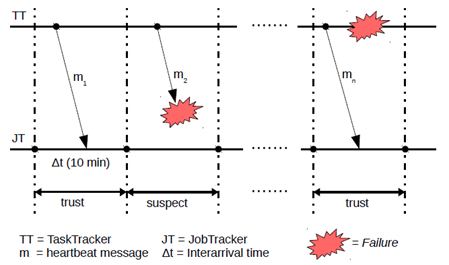
\includegraphics[width=12cm]{./image/tasktracker.png}}
\caption{TaskTracker Failure Detection Model in Hadoop Framework \cite{adaptiveScheduling}}\label{fig:tasktracker}
\end{figure}

For example, active TaskTracker send heartbeat messages to JobTracker every 3 seconds.  While JobTracker check the timeout condition every 200 seconds.  And there are network delays or messages losses, so some heartbeat may arrive late or loss.  The JobTracker may consider that TaskTracker as dead node even it is available as shown in Figure~\ref{fig:tasktracker}. that heartbeat message m2 does not arrive and the JobTracker consider this TaskTracker as dead.

\newpage
\subsection{Container Technology}
\begin{figure}[!h]\centering
\setlength{\fboxrule}{0mm} % can define this in the preamble
\setlength{\fboxsep}{0cm}
\fbox{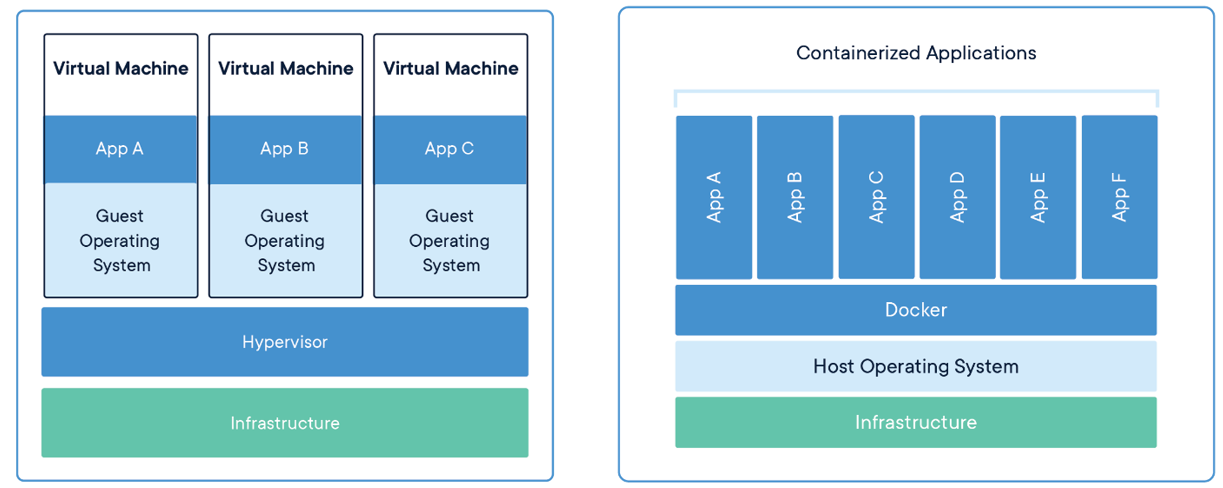
\includegraphics[width=13cm]{./image/vmVSContainer.png}}
\caption{Virtual machine vs Container \cite{docker}}\label{fig:vmVSContainer}
\end{figure}
Container Technology is a method to package up code and all its dependencies, so the application runs quickly and reliably from one computing environment to another, with container software having names including the popular choices of Docker, Apache Mesos, RKT, and Kubernetes.  The virtual machine contains the entire operating system.  Therefore, the physical server that runs several virtual machines is running several operating systems’ simultaneously as shown in Figure~\ref{fig:vmVSContainer}. \cite{docker}

There is a lot of overhead on virtual machine.  In contrast, with container technology, the server runs a single operating system.  Each container can share this single operating system with other containers on server.  Containers require less resource of server with less overhead and more efficient than virtual machines. \cite{container}   Containers are set up to accomplish work in a multiple container architecture (container cluster).  They also enable a program to be broken down into smaller pieces, which are known as microservices.  So, the program can work on each of the containers separately.

\subsection{Overview of machine learning}
Machine learning is a branch of artificial intelligence (AI).  It is the machine’s ability to learn from data provided without human intervention and able to improve decision from experience.  Without human directed programming instructions, the machine accesses data, observes and finds data pattern.  The more data input the better data pattern learning and better decision making.\cite{ml}

\subsection{Overview of machine learning}
An artificial neural network (ANN) is a computational model imitates the natural human brain. The network consists of hundreds or thousands small neuron nodes. Those numerous neuron nodes communicate to each other in the web form. The neuron node is called processing unit. Each of processing unit is interconnected by nodes. Each processing unit comprises of input unit and output unit. Input unit receives various type of data format. It also has an internal weighting system. The neural network learns from the input and produce output result.

ANN use rules and guidelines to generate result/ output. The set of these learning rules is called backpropagation because it uses backward propagation of error to learn or improve the better result. ANN learns data patterns in training phase. It compares actual output with the desired output that is expected result in supervised phase. The difference between actual and expected result are worked backward to adjust the weight of its connections between the units. The purpose is to make the lowest possible error. \cite{ann}

\subsection{Deep learning}
Nowadays, there are collections of vast unlabeled and unstructured data gathering from various sources that is difficult to analyses useful information by traditional programs in a linear way.  The hierarchical level of artificial neural network that work in web form to process data with a nonlinear approach is called Deep Learning.  The first layer of the neural network processes a raw data and pass output on to the next layer. The second layer processes first layer output plus additional information and pass output to next layer again. This continues across all levels of the neuron network to make information more meaningful information. \cite{deepLearning}

Deep learning models can achieve high accuracy, sometimes exceeding human-level performance. “Deep” refers to the powerful number of hidden layers in the neural network.  However, it needs lots of labeled data and high-performance machines to analyze. The organized layers of interconnected nodes can be tens or hundreds of hidden layers. \cite{deepLearning2} as shown in Figure~\ref{fig:NN}.

\begin{figure}[!h]\centering
\setlength{\fboxrule}{0mm} % can define this in the preamble
\setlength{\fboxsep}{0cm}
\fbox{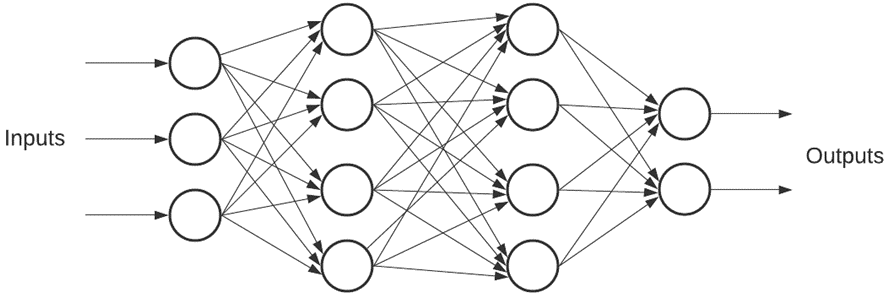
\includegraphics[width=8cm]{./image/NN.png}}
\caption{Neural networks.}\label{fig:NN}
\end{figure}

\newpage
\section{Technologies survey}  
\subsection{Apache Mesos}
Mesos consists of a master, agent daemons running on each cluster node, and Mesos frameworks that run task on these agents as shown in Figure~\ref{fig:MesosArc}. Architecture consist of three components: masters, slaves, and the frameworks that run on them. Mesos relies on Apache ZooKeeper, a distributed database used specifically for coordinating leader election within the cluster, and for leader detection by other Mesos masters, slaves, and frameworks. \cite{mesosInAction}

\begin{figure}[!h]\centering
\setlength{\fboxrule}{0mm} % can define this in the preamble
\setlength{\fboxsep}{0cm}
\fbox{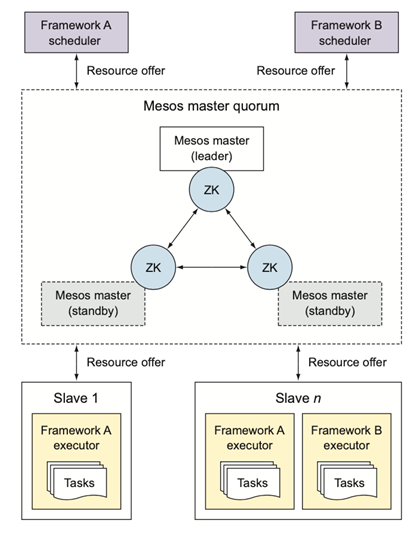
\includegraphics[width=10cm]{./image/MesosArc.png}}
\caption{The Mesos architecture consists of one or more masters, slaves, and frameworks. \cite{mesosInAction}}\label{fig:MesosArc}
\end{figure}

\begin{enumerate}
  \item \textbf{Masters: } Mesos masters are responsible for managing the Mesos slave daemons running on each machine in the cluster. Using Zookeeper, they coordinate which node will be the leading master, and which masters will be on standby, and ready to take over if the leading master goes offline. A Mesos cluster requires minimum one master, and three or more are recommended for production deployments. Zookeeper can run on the same machines as the Mesos masters themselves or use a standalone Zookeeper cluster. 
  \item \textbf{Slaves: } The machines in a cluster responsible for executing a framework’s tasks.
  \item \textbf{Frameworks: } Mesos application that’s responsible for scheduling and executing tasks on a cluster. A framework is made up of two components: a scheduler and an executor. 
  \begin{itemize}
     \item \textbf{Schedulers} A scheduler is a long-running service responsible for connecting to a Mesos master and accepting or rejecting resource offers. Mesos delegates the responsibility of scheduling to the framework, instead of attempting to schedule all the work for a cluster itself. The scheduler can then accept or reject a resource offer based on whether it has any tasks to run at the time of the offer. 
     \item \textbf{Executor} An executor is a process launched on a Mesos slave that runs a framework’s tasks on a slave.
   \end{itemize}
\end{enumerate}

Dominant resource is a resource of specific type (CPU, memory, disk, ports) which is most demanded by given framework among other resources it needs. DRF computes the share of resource allocated to a framework (dominant share) and tries to maximize the smallest dominant share in the system. for next round offers the resources first to the one with smallest dominant share, then to the second smallest one and so on. \cite{drf} Example with 9 CPUs and 18 GB RAM to two frameworks running task that require <1 CPU, 4GB> and <3CPUs, 1GB> shown in Table~\ref{tbl:DRFTwoFramework}.

\begin{table}[!h]
\caption{Example of running 2 frameworks.}\label{tbl:DRFTwoFramework}
\begin{tabular}{|c|c|c|c|c|c|c|}
\hline
\multirow{2}{*}{Schedule} & \multicolumn{2}{c|}{Framework A}& \multicolumn{2}{c|}{Framework B}& \multicolumn{2}{c|}{total}\\ 
\cline{2-7} & Resource Share & Dominant Share & Resource Share & Dominant Share & CPU & RAM \\ 
\hline
B  & <0, 0> & 0 & <3/9, 1/18> & 1/3 & 3/9 & 1/18 \\ 
\hline
A  & <1/9>, <4/18> & \textbf{2/9} & <3/9, 1/18> & 1/3 & 4/9 & 5/18 \\ 
\hline
A  & <2/9>, <8/18> & 4/9 & <3/9>, <1/18> & \textbf{1/3} & 5/9 & 8/18 \\ 
\hline
B  & <2/9>, <8/18> & \textbf{4/9} & <6/9>, 2/18> & 2/3 & 8/9 & 10/18 \\ 
\hline
A  & <3/9>, <12/18> & 2/3 & <6/9>, 2/18> & 2/3 & 1 & 14/18 \\ 
\hline
\end{tabular}
\end{table}

\subsection{Zookeeper}
ZooKeeper is an open-source Apache project that provides a centralized service for providing configuration information, naming, synchronization, and group services over large clusters in distributed systems. The goal is to make these systems easier to manage with improved, more reliable propagation of changes. ZooKeeper provides an infrastructure for cross-node synchronization by maintaining status type information in memory on ZooKeeper servers. A ZooKeeper server keeps a copy of the state of the entire system and persists this information in local log files. Large Hadoop clusters are supported by multiple ZooKeeper servers, with a master server synchronizing the top-level servers. \cite{zookeeper}

\subsection{Elasticsearch}
Elasticsearch is an open-source search and analytics engine built on Apache Lucene and developed in Java. Elasticsearch can be used to store and search all kinds of documents, analyze huge volumes of data in near real-time and give back answers in milliseconds, and supports multitenancy. It’s able to achieve fast search responses because it searches an index directly instead of searching the text. Related data is often stored in the same index, which consists of one or more primary shards, and zero or more replica shards. Once an index has been created, the number of primary shards cannot be changed. It uses a structure based on documents and comes with extensive REST APIs for storing and searching the data. 

Elasticsearch is the component of the Elastic Stack, a set of open-source tools for storage, analysis, and visualization. The four components, Elasticsearch, Logstash, Kibana and Beats, are designed for use as an integrated solution. It is commonly referred to as the “ELK” stack.\cite{elasticsearch}

\subsection{Chronos}
Chronos is the Mesos Cron system. It handles time-based scheduling of jobs on a Mesos cluster. Chronos can be used to schedule commands or scripts. The Chronos feature set is easily and reliably to create standalone schedule-based jobs, as well as complex dependency-based jobs and pipelines, simply by specifying the schedule and resources that the job requires. This guarantees that time-based jobs are running on time while continuing to use datacenter resources as efficiently as possible. In Figure~\ref{fig:chronos}, it shows about the differences between running Cron jobs on a single machine and running them on a Mesos cluster.\cite{mesosInAction}

\begin{figure}[!h]\centering
\setlength{\fboxrule}{0mm} % can define this in the preamble
\setlength{\fboxsep}{0cm}
\fbox{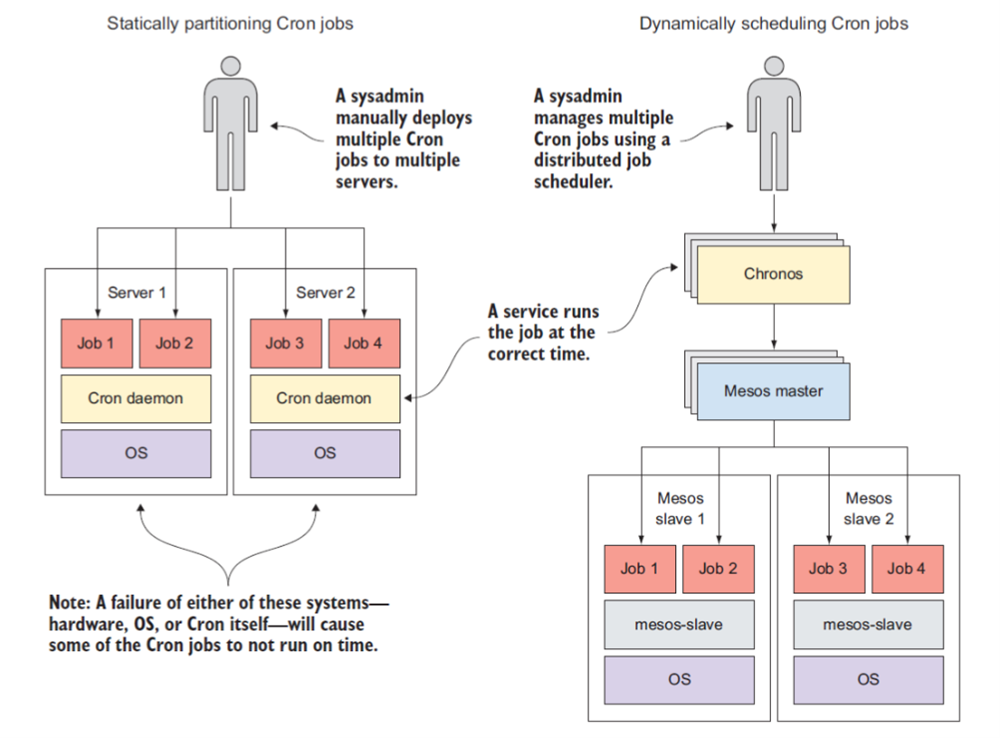
\includegraphics[width=10cm]{./image/chronos.png}}
\caption{Mesos and Chronos provide a dynamic, fault-tolerant environment to run time-based jobs. \cite{mesosInAction}}\label{fig:chronos}
\end{figure}

\subsection{Marathon}
Marathon is a popular open source Mesos framework developed by Mesosphere. Marathon is used for deploying long-running services and applications, both in Linux cgroups and Docker containers. It can also be considered a private platform as a service (PaaS) on which to deploy applications. Marathon can specify the resources needed for each instance of an application and number of running instances. If a Mesos slave fails, or an instance of application crashes or exits, Marathon will automatically start a new instance to replace the failed one.

Marathon also allows users to specify dependencies on other services and applications during deployment, so an application instance can’t start before its database instance is up and passing health checks. Marathon contains a list of features that should satisfy the needs of most application management scenarios such as managing applications and groups of applications with dependencies and health checks, rolling application upgrades with specific capacity requirements, a powerful web interface and REST API, and high availability (using ZooKeeper for leader election and coordination).\cite{mesosInAction}

\subsection{Spark}
Apache Spark, unified analytics engine for large-scale data processing, runs on Hadoop, Apache Mesos, Kubernetes, standalone, or in the cloud. It can access diverse data sources. Spark perform task faster and more efficiently than Hadoop’s MapReduce, both in memory and on disk in many cases. Spark also provide API for several programming language, including Python, Scala and Java and support streaming workloads, interactive queries and machine learning libraries, in addition to MapReduce-like batch processing.  Spark can run locally. But that is useful only for development purpose, the number of CPU cores limits the number of executors. When setting up a production Spark cluster, there are two option.

When setting up statically partitioned cluster on an Infrastructure as a Service (IaaS) provider. It will be wasting money due to cloud instances sitting idle. Find-grained resource sharing can help increase system’s utilization. For example, if there are two applications likes in Figure~\ref{fig:spark}, Spark and Jenkins that need to run on multiple servers. Each of these system atop a general-purpose cluster manager like Mesos that allows for this sort of fine-grained resource sharing. It can share compute resources and run multiple workloads on a single Mesos slave. This will lead to better resource utilization across many machines within a modern datacenter.\cite{mesosInAction}

\begin{figure}[!h]\centering
\setlength{\fboxrule}{0mm} % can define this in the preamble
\setlength{\fboxsep}{0cm}
\fbox{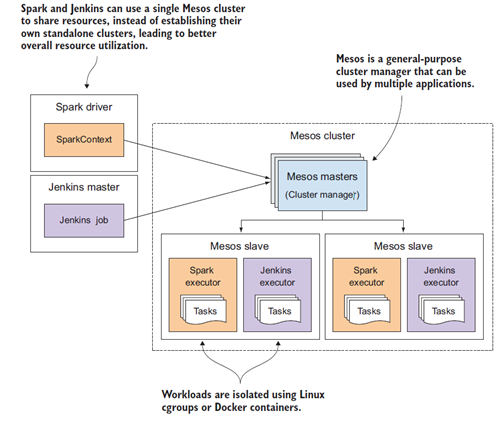
\includegraphics[width=10cm]{./image/spark.png}}
\caption{Mesos managing cluster resources for two applications. \cite{mesosInAction}}\label{fig:spark}
\end{figure}

\subsection{Apache Kafka}
Apache Kafka is an open-source stream-processing software platform. Apache Kafka is providing a unified, high-throughput, low-latency platform for handling real-time data feeds. Kafka allows user to subscribe itself and publish data to any number of systems or real-time applications. In Figure~\ref{fig:kafka}, producers are processes that send message to Kafka. Then, Kafka stores these messages in key-value. The data can be partitioned into different topic. And Consumers are process that can read messages from partitions. Kafka runs on a cluster of one or more server, And the topics are distributed across the cluster nodes. And partitions are replicated to multiple servers.\cite{kafka}

\begin{figure}[!h]\centering
\setlength{\fboxrule}{0mm} % can define this in the preamble
\setlength{\fboxsep}{0cm}
\fbox{
\includegraphics[width=10cm]{./image/kafka.png}}
\caption{Overview of Kafka. \cite{kafka}}\label{fig:kafka}
\end{figure}

\section{Related Research}
The current data center management is a representative large-scale resource management and scheduling framework for clusters, liked the open-source project Mesos \cite{mesosInAction}. However, the data center environment are cluster systems and variety of submitted tasks, such as Hadoop clusters that support big data processing and Spark clusters that support in-memory computing. Mesos is a resource allocation method with no differential task type and scheduler does not consider the overall resource demand or workload, which leads to low average resource utilization and starve were a framework with a high demand on queue. Moreover, Mesos uses the DRF (Dominant Resource Fairness) algorithm for resource allocation. The DRF algorithm is the default scheduling algorithm of Mesos, the algorithm still has the disadvantage of not considering the machine performance and task type.

Many researchers have conducted relevant work. For example, in 2016, Li Y et al \cite{fishSwarm} introduced the fish swarm intelligence algorithm to dynamically adjusting the Mesos cluster resources to improve the Mesos load imbalance and resource utilization. The DRF scheduling algorithm of Mesos is extended, and in 2018, Wenbin Liu et al. proposed A X-DRF algorithm \cite{xdrf} based on building classifies the performance of physical machines and job type judgment classification is proposed to solve the problem of machine performance in literature, but the task type is not considered and not consider the waiting time. Compared with the original DRF algorithm, the X-DRF algorithm has higher system resource utilization rate, which is in line with the actual production rules of data centers, and provides new ideas for heterogeneous cluster multi- resource management for data center managers. In 2019, Pankaj Saha et al. developed Tromino \cite{tromino}, a policy driven queue manager. Tromino allows task from individual frameworks to be scheduled based on each framework’s overall resources requirement and current resources consumption. Tromino reduce the impact of unfairness due to framework specific configuration and unfair waiting time due to higher resource demand in a pending task queue.

%%%%%%%%%%%%%%%%%%%%%%%%%%%%%%%%%%%%%%%%%%%%%%%%%%%%%55
%%%%%%%%%%%%%%%%%%%%%%%%%%%%%%%%%%%%%%%%%%%%%%%%%%%%%
%%%%%%%%%%%%%%%%%%%%%%%%%%%%%%%%%%%%%%%%%%%%%%%%%%%%%
\chapter{Proposed Work}

Explain the design (how you plan to implement your work) of your project. Adjust the section titles below to suit the types of your work. Detailed physical design like circuits and source codes should be placed in the appendix.

\section{System Architecture}

\begin{table}[!h]
\centering
\caption{test table x1}\label{tbl:symbols}
\begin{tabular}{@{}p{0.07\textwidth}|p{0.7\textwidth}p{0.1\textwidth}}\hline
\multicolumn{2}{l}{\textbf{SYMBOL}}  & \textbf{UNIT} \\ \hline 
$\alpha$ & Test variable\hfill & m$^2$ \\
$\lambda$ & Interarrival rate\hfill &  jobs/second\\
$\mu$ & Service rate\hfill & jobs/second \\ \hline
\end{tabular}
%\begin{tabular}{c|c} \hline
% $\alpha$ & $\beta$ \\ \hline
% $\delta$ & $\mu$ \\ \hline
%\end{tabular}
\end{table}

\section{System Specifications and Requirements}

\section{Hardware Module 1}
\subsection{Component 1}
\subsection{Logical Circuit Diagram}

\section{Hardware Module 2}
\subsection{Component 1}
\subsection{Component 2}

\section{Path Finding Algorithm}

\section{Database Design}

\section{GUI Design}



%%%%%%%%%%%%%%%%%%%%%%%%%%%%%%%%%%%%%%%%%%%%%%%%%%%%%%%%%%%%%%
%%%%%%%%%%%%%%%%%%%% Experiments %%%%%%%%%%%%%%%%%%%%%%%%%%%%%
%%%%%%%%%%%%%%%%%%%%%%%%%%%%%%%%%%%%%%%%%%%%%%%%%%%%%%%%%%%%%%%
\chapter{Implementation Results}

You can title this chapter as \textbf{Preliminary Results} or \textbf{Work Progress} for the progress reports. Present implementation or experimental results here and discuss them.

%%%%%%%%%%%%%%%%%%%%%%%%%%%%%%%%%%%%%%%%%%%%%%%%%%%%%%%%%%%%%%%
%%%%%%%%%%%%%%%%%%%% Conclusions %%%%%%%%%%%%%%%%%%%%%%%%%%%%%
%%%%%%%%%%%%%%%%%%%%%%%%%%%%%%%%%%%%%%%%%%%%%%%%%%%%%%%%%%%%%%%
\chapter{Conclusions}

This chapter is optional for proposal and progress reports but 
is required for the final report.

\section{Problems and Solutions}
State your problems and how you fixed them.

\section{Future Works}
What could be done in the future to make your projects better.

%%%%%%%%%%%%%%%%%%%%%%%%%%%%%%%%%%%%%%%%%%%%%%%%%%%%%%%%%%%%%%%
%%%%%%%%%%%%%%%%%%%% Bibliography %%%%%%%%%%%%%%%%%%%%%%%%%%%%%
%%%%%%%%%%%%%%%%%%%%%%%%%%%%%%%%%%%%%%%%%%%%%%%%%%%%%%%%%%%%%%%

%%%% Comment this in your report to show only references you have
%%%% cited. Otherwise, all the references below will be shown.
\nocite{*}
%% Use the kmutt.bst for bibtex bibliography style 
%% You must have cpe.bib and string.bib in your current directory.
%% You may go to file .bbl to manually edit the bib items.
\bibliographystyle{kmutt}
\bibliography{string,cpe}





\end{document}
